\begin{question}
\noindent Triangle $A$ is reflected in the line $y = x - 1$ to give triangle $A'$, as shown on the grid below.

\begin{center}
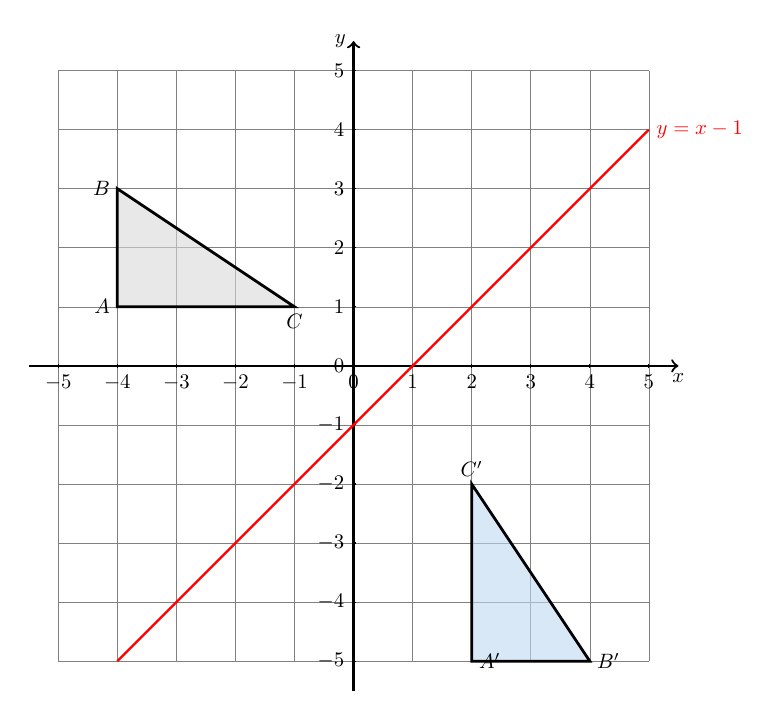
\begin{tikzpicture}[scale=0.75, transform shape]
    % Define colours
    \definecolor{borderColour}{HTML}{000000}
    \definecolor{fillColourA}{HTML}{D8D8D8}
    \definecolor{fillColourAp}{HTML}{BFD9F2}

    % Define axis scale
    \def\axisLimit{5}

    % Draw grid
    \draw[step=1cm,gray,very thin] (-\axisLimit,-\axisLimit) grid (\axisLimit,\axisLimit);

    % Draw axes
    \draw[thick,->] (-\axisLimit-0.5,0) -- (\axisLimit+0.5,0) node[anchor=north] {$x$};
    \draw[thick,->] (0,-\axisLimit-0.5) -- (0,\axisLimit+0.5) node[anchor=east] {$y$};

    % Label x-axis and y-axis
    \foreach \x in {-\axisLimit,...,\axisLimit}
        \draw (\x cm,1pt) -- (\x cm,-1pt) node[anchor=north] {$\x$};
    \foreach \y in {-\axisLimit,...,\axisLimit}
        \draw (1pt,\y cm) -- (-1pt,\y cm) node[anchor=east] {$\y$};

    % Mirror line y = x - 1
    \draw[thick, red] (-4,-5) -- (5,4) node[right] {$y = x - 1$};

    % Triangle A
    \coordinate (A) at (-4,1);
    \coordinate (B) at (-4,3);
    \coordinate (C) at (-1,1);
    \filldraw[fill=fillColourA, draw=borderColour, line width=1pt, fill opacity=0.6] (A) -- (B) -- (C) -- cycle;
    \node[left] at (A) {$A$};
    \node[left] at (B) {$B$};
    \node[below] at (C) {$C$};

    % Triangle A' (reflection of A in y = x - 1)
    \coordinate (A') at (2,-5);
    \coordinate (B') at (4,-5);
    \coordinate (C') at (2,-2);
    \filldraw[fill=fillColourAp, draw=borderColour, line width=1pt, fill opacity=0.6] (A') -- (B') -- (C') -- cycle;
    \node[right] at (A') {$A'$};
    \node[right] at (B') {$B'$};
    \node[above] at (C') {$C'$};

\end{tikzpicture}
\end{center}

\noindent A gamer is designing a symmetric map layout in Valorant using this reflection as a template. Points that do not move under the reflection are needed to place a fixed spawn structure.

Find the coordinates of the point(s) on triangle $A$ that map to themselves (invariant points) under this reflection.

\vspace{4cm}

\begin{flushright}
    \answerplain{3}
\end{flushright}
\end{question}
